%%%% -*- mode: Latex; TeX-master: "nrt16.tex"; -*-
\documentclass[11pt]{article}

\vspace{10pt}

\usepackage{fullpage,times,subfigure,fancyhdr}
\usepackage[pdftex]{color}
\usepackage{xcolor}
\usepackage{hyperref}
\usepackage{wrapfig}
\usepackage{textcomp}
\usepackage{verbatim}
\usepackage{cite}
\usepackage{times}
\usepackage{amsfonts,amsmath,amssymb,amsthm}
\usepackage{textcomp}
\usepackage{url}
\usepackage{mdwlist}
\usepackage{subfigure}
\usepackage{wrapfig}
\usepackage{xspace}
\usepackage[pdftex]{graphicx}
\usepackage{setspace}
\usepackage{hyperref}
\usepackage{enumitem}
\usepackage{colortbl}

\definecolor{bl}{rgb}{0.,0.2,0.6}
\definecolor{dark_blue}{rgb}{0,.15,.5}
\usepackage[linecolor=dark_blue, linewidth=1.5pt, skipabove=4pt, nobreak=true]{mdframed}

\newcommand{\db}[1]{{\color{dark_blue}{#1}}}
\newcommand{\bb}[1]{{\textbf{\db{#1}}}}

\newcommand{\rb}[1]{{\color{red}{\it [RB: #1]}}}
\newcommand{\tz}[1]{{\color{green}{\it [TZ: #1]}}}
\newcommand{\lb}[1]{{\color{blue}{\it [LB: #1]}}}
\newcommand{\jovo}[1]{{\color{lime}{\it [JoVo: #1]}}}
\newcommand{\mr}[1]{{\color{teal}{\it [MR: #1]}}}
\newcommand{\as}[1]{{\color{violet}{\it [AS: #1]}}}
\newcommand{\ya}[1]{{\color{lime}{\it [YA: #1]}}}
\newcommand{\je}[1]{{\color{brown}{\it [JE: #1]}}}


\newcommand{\sectn}[1]{\section{#1} \rfoot{\small #1 ~~ \thepage}}
%\newcommand{\sectn*}[1]{\section*{#1} \rfoot{\small #1 ~~ \thepage}}


\renewcommand{\thepage}{\thesection-{\arabic{page}}}
\renewcommand{\thesection}{\Alph{section}}   % set the section counter to Alpha
\renewcommand{\thesubsection}{\Alph{section}.\arabic{subsection}}   % set the subsection counter to alpha
\renewcommand{\thesubsubsection}{\Alph{section}.\arabic{subsection}(\arabic{subsubsection})}

\newcommand\weblink[1]{\underline{\textcolor{dark_blue}{#1}}}

\usepackage{titlesec}

\titleformat{\section}
{\color{dark_blue}\normalfont\Large\bfseries}
{\color{dark_blue}\thesection}{1em}{}
\titlespacing*{\section}{0pt}{0pt}{4pt}

\titleformat{\subsection}
{\color{dark_blue}\normalfont\large\bfseries}
{\color{dark_blue}\thesubsection}{1em}{}
\titlespacing*{\subsection}{0pt}{7pt}{3pt}

\titleformat{\subsubsection}
{\color{dark_blue}\normalfont\large\bfseries}
{\color{dark_blue}\thesubsubsection}{1em}{}
\titlespacing*{\subsubsection}{0pt}{8pt}{4pt}

\newcommand{\para}[1]{\vspace{5pt}\noindent{\bb{\bf #1:}}}
\newcommand{\paranc}[1]{\vspace{5pt}\noindent{\bb{\bf #1}}}

\pagestyle{fancy}
\lhead{}
\chead{}
\rhead{}
\lfoot{}
\cfoot{}
\rfoot{}
\renewcommand{\headrulewidth}{0pt}
\renewcommand{\footrulewidth}{0pt}

\newcommand{\idies}{{Institute for Data-Intensive Science and Engineering, Johns Hopkins University}}
\newcommand{\jhu}{{Johns Hopkins University}}

\usepackage{pifont}
\usepackage{xspace}
\newcommand{\circone}{\ding{172}\xspace}
\newcommand{\circtwo}{\ding{173}\xspace}
\newcommand{\circthree}{\ding{174}\xspace}
\newcommand{\circfour}{\ding{175}\xspace}

\tolerance=1000

%\addtolength{\textfloatsep}{-10pt}

%\renewcommand{\topfraction}{0.99}
%\renewcommand{\textfraction}{0.10}
%\renewcommand\floatpagefraction{0.99}
%\renewcommand{\subfigcapskip}{0pt}

\makeatletter
\renewcommand{\labelitemi}{*}

\title{Brain Comp Infra: EAGER: BrainLab CI: Collaborative, Community Experiments with Data-Quality Controls through Continuous Integration}

\author{{Randal Burns (PI) }\\
         {\small Department of Computer Science} \\
         \\
         Joshua T. Vogelstein and Michael I. Miller\\
         {\small Department of Biomedical Engineering}\\
          \\
         {\bf Kavli Neuroscience Disovery Institute}
         { \bf Johns Hopkins University } \\
}



%\addtolength{\textfloatsep}{-20pt}

\tolerance=500

\begin{document}



\maketitle
\thispagestyle{empty}

\begin{center}
\large
 Proposal to the National Science Foundation \\
 Program Solicitation NSF DCL 16-706--- National Science Foundation Brain Computational Infrastructure \\

\end{center}

\newpage

\makeatletter

\tolerance=500

\setcounter{page}{1}
\setcounter{section}{1}
\sectn{PROJECT SUMMARY}

\normalsize


The BrainLab CI prototype system will deploy an experimental-management infrastructure that allows users to construct community-wide experiments that implement data and metadata controls on the inclusion and exclusion of data. It will do so by building upon the principle of continuous integration (CI), adopted from the agile software development community. The CI platform allows the designer of an experiment to place multiple simple or complex controls on data, such as requiring specific metadata, that data are registered to a given atlas, or that data are collected using specific experimentation protocols. Controls may include reprocessing data to make it compliant, e.g. reregistering MRI data to a given atlas or band-pass filtering electrophysiology data. Controls and processing will run user-defined scripts and programs within a software container (e.g., Docker) on a serverless computing cloud, such as Amazon Lambda. Containers encapsulate all dependencies to ensure that software runs uniformly against all inputs on all platforms. Serverless computing automatically and elastically provisions cloud resources to run containers.

BrainLab CI will create a meaningful way to scale science from the tens of subjects used by individual labs today to thousands or tens of thousands, while allowing scientists to exert controls that ensure data quality, initially with two different experimental patterns: (1) An incremental experiment defines an experiment against a existing data set and then opens the experiment to community contributions. Other labs/scientists contribute data which gets processed on submission and included or rejected. The experiment maintains online dashboards that show how additional data change results with complete provenance. (2) A derived experiment forks/branches an existing experiment allowing a researcher to change properties, such as an acceptance criteria or analysis algorithm, but otherwise run the same pipeline against the same inputs. Full provenance allows scientists to reason and debate about how modifications affect outcomes. These patterns can be composed and the fork/branch version control model of the CI system connects changes in experiments to outcomes. We will co-develop community experiments for MRI and for neurophysiology (including both optical and electrical physiology); these domains were chosen because they are critical to NSF BRAIN neuroscience, have large bodies of unshared data living in silos in different labs, and they produce large numbers of relatively small (GB-scale) data sets that are managed easily in a prototype.

\para{Broader Impacts} 
%
BrainLab CI has the potential to permanently transform practice in neuroscience. The design principles for the system grew out of the NSF KAVLI Global Brain Workshop's discussion on realizing a global-shared infrastructure for scientific discovery. BrainLab CI overcomes major obstacles to data sharing. It does not restrict scientists to a specific workflow system, ontologies, software frameworks, etc. Rather, scientists package their custom experiments into containers and set admission criteria for new data. Scientists share data without losing control over data quality; they gain full provenance on how all subsequent experiments use their data and algorithms. This provenance can be used to debate and reason about different results from the same data or how specific data changes affect results. With these important barriers to data sharing removed, we envision a system that meaningfully integrates the 1000s of publicly available data resources in MRI and neurophysiology and creates incentives for data sharing for individual labs and data collectors, who gain great analytic power by confronting their new data with a massive corpus.

\para{Intellectual Merit} 
%
BrainLab CI adopts cutting-edge practice in agile software development and cloud computing to build a totally unique capability for neuroscience. By adopting containers, which encapsulate all software dependencies, and serverless computing, we will create an automated system that runs arbitrary and sophisticated checks on submitted data. Data contributors experience no overhead: they upload a data set via file transfer or Web service and the system automatically runs the continuous integration suites. Experiment designers write simple programs, e.g. scripts, or complex workflows to express their constraints and continuous integration enforces these automatically and at scale.

\vspace{-3pt}



\newpage

\setcounter{section}{3}
\setcounter{page}{1}
\sectn{PROJECT DESCRIPTION}


\noindent The brain research community desperately needs to build shared infrastructure that combines the many publicly available imaging data sets and allows researchers to define and conduct experiments that confront thousands or tens-of-thousands of subjects, rather than the tens used today by individual labs. Scientists will gain great analytical power by referencing their studies against a massive corpus, allowing them to focus on experimental design and data analysis, rather than data collection. This will engage a national and international community of researchers that do not collect---an expensive activity limited to few labs. It will also drive a change in scientific culture, encouraging data sharing, the development of common analysis tools, and accelerated discovery from connecting ideas, tools, data, and people.

Data quality and data control present major obstacles to successful data sharing and to participation. Bad data leads to bad science and data collectors and the neuroscience community are legitimately concerned about the misuse of data. To be useful in a shared infrastructure, datasets need to have sufficient metadata and employ collection, preparation, and data processing protocols that produce comparable data. Examples include stimulus in functional MRI studies or cell type and sample preparation for single-cell spike-train data. For a shared infrastructure to be transformative, it needs to link experiments to data, allow data providers to exert control on how data are used and what data can be included in a study, and allows data consumers to define and customize experiments consistent with exploratory analysis and data mining.

We propose a platform to define ongoing, incremental, and community experiments with data controls based on the agile software development principle of {\em continuous integration} (CI). In CI, every time new source is committed, it is automatically built against a suite of tests and multiple configurations and deployed with the goals of keeping all contributions merged, maintaining a single view of the repository, and keeping deployed software updated. We propose an analogous workflow for neuroscience experiments in which (1) the community contributes new data incrementally to an experiment and (2) scientists derive and customize new virtual experiments that inherit existing data and data controls. 

The resulting {\em BrainLab CI} will take existing studies and provide a continuously updated view that integrates the latest results, couples changing results to new data, and provides dashboards that link outcomes to input data.  Experiment maintainers gain provenance for outcomes and can
 refine data controls.
An incremental community experiment will build on an established result, extending its scope and power. Researchers will seed the repository with reviewed and published results by pushing an experiment and a dataset to the BrainLab CI repository, for example, an Alzheimer’s study that links the shape of the Amygdala with functional MRI that produces a classifier that identifies diseased brains with a given accuracy and significance (p-value). The research will include scripts and programs that implement data controls that describe the data selection criteria: (1) requiring that shape data are registered to a given atlas, potentially running a registration pipeline for non-conforming data and accepting/rejecting data based on the result; (2) checking for metadata that describes a compatible imaging protocol, such as duration and stimulus; and, (3) validates that fMRI data were processed with a given pipeline (CPAC \cite{cpac}, FSL \cite{fsl}), reprocessing the data into this form when possible. This experimental definition provides a base version and checkpoint that links the data set with the published result and repeatedly computes the published result in BrainLab CI.

Additional data sets are added to the experiment in batches or incrementally. Our example experiment may link to the thousands of compatible brains stored in MRICloud (\url{http://mricloud.org}). The outcome of linking will include updated experimental results based on the new data and a description of which data passed controls and why data were rejected. A continuous {\em community experiment} will accept new imaging raw data incrementally, registering and pre-processing it as part of data controls, and maintain an up-to-date view of outcomes as data changes. Each contribution defines a new experiment that has provenance, linking results to the source data. Analysis dashboards allow all to look at how results vary based on the inclusion/exclusion of different data. Controls may be added or removed to create experimental variants that reveal the structure of an outcome.

BrainLab CI inherits the fork/clone model of software repositories, allowing scientists to vary experiments and inherit from existing experiments. Experimental variants document the data controls so that researchers can reason about and dispute divergent findings and link the divergence to selection criteria, algorithms, etc. In our example, we may include diffusion MRI data and study the tradeoff in classification between adding a new imaging modality and reducing the number of subjects. A scientist exploring bias/variance tradeoffs would {\em fork} an existing experiment and change data selection criteria. The results would be directly comparable to the original and new data could be added to both experiments independently.
The fork/clone/versioning model when combined with container-based computing (see Technology) guarantees repeatability and reproducibility. 
Programmatic data selection against online repositories create data provenance, specifying the exact inputs.  The experimental version links data to an outcome.  And, because we run in containers, the same program produces exactly the same output on future and legacy systems.

\subsection{Reference Applications}
\label{sec:apps}

At the EAGER scale, BrainLab CI targets two neuroscience problem domains: (1) multimodal (structural, functional, and diffusion) MRI imaging studies linked with shape, genomic, and phenotypic information and (2) neurophysiology data linked with cell type, genomic, and computational neuroscience models.  Both domains have a large body of unshared data from many labs that are currently incomparable.  Both produce large numbers of relatively small (GB) data sets that can be combined in a modest computational infrastructure.  Furthermore, both  were identified as ideal candidates for sharing in the recent NSF KAVLI Global Brain Workshop.

\subsubsection{Brainlab MRI}

% Desribe a community experiment and an example dashboard.
An MRI experiment may consist of a diffusion and structural scan for a number of subjects using a novel set of scanning parameters.  The data could be stored in a standard format accepted by many public repositories (\url{http://bids.neuroimaging.io/}) and ingested into the NeuroData system.  Then, nonlinear image registration would warp the data to a common atlas of the user's choosing (currently, NeuroData stores over 24 atlases; \url{http://docs.neurodata.io/nddocs/mrgraphs/atlases.html}), followed by tensor estimation, tractography, and network estimation.  The experimentalist may then seek to understand how the images generating under this new scanner sequence look as compared with previously existing sequences. Because many different datasets are stored in the same format, linking to others is easy.  Figure \ref{f:mri} shows one of the many possible different summary statistics across eight different datasets, demonstrating significant batch effects for the KKI2009 data: its values are an order of magnitude higher than for the other datasets; checking the metadata reveals that KKI2009 used a different MRI machine than the other datasets in this comparison.


\subsubsection{Brainlab Physiology}

A typical experiment from calcium imaging may proceed as follows.  Image data are stored in a pre-determined general specification (for example, images stored according to the NeuroData specification \url{http://docs.neurodata.io/ndstore/sphinx/ingesting.html}), ingested into the system, cell bodies are automatically detected, followed by spike detection, and then network estimation.  In addition to the physiology data, there will also typically be metadata, which could be stored according to the Neurodata without Borders specification \url{http://www.nwb.org/resources/}. A single experiment might include multiple trials per ``run'', with multiple runs per animal, and multiple animals.  For example, the trial specific metadata may be a time-varying visual stimuli for an anesthetized animal. In such a scenario, the experimentalist may desire to condition the network estimation on the stimuli, and look at the statistical network differences across conditions.

Under such a scenario, the dashboard may provide certain per run visualizations as depicted in Figure \ref{f:wilcox} (top three panels). Next, it may show summary statistics for said run (next panel).  Finally, it could show the statistical comparisons pooling over all animals in the experiment (bottom panel).

In this experiment, of course, there are many different variables that different experimentalists may want to consider, or even the same experimentalist may want to consider at different times.  For example, as new and improved spike detection tools become available \cite{Vogelstein2010b}, users will want to swap out the old and swap in the new.  Of note, if other people had also collected data from the same neurons (say, in an invertebrate species), with overlapping stimulus conditions, it would be easy to also pool that data. Finally, while this entire experiment has been discussed in the context of optophysiology based on calcium imaging, the number of changes required if one were to fork this to apply it to fMRI data are quite minimal, because of the common interface to data across modalities, laboratories, and experiments.


\begin{figure}%{l}{0.5\textwidth}
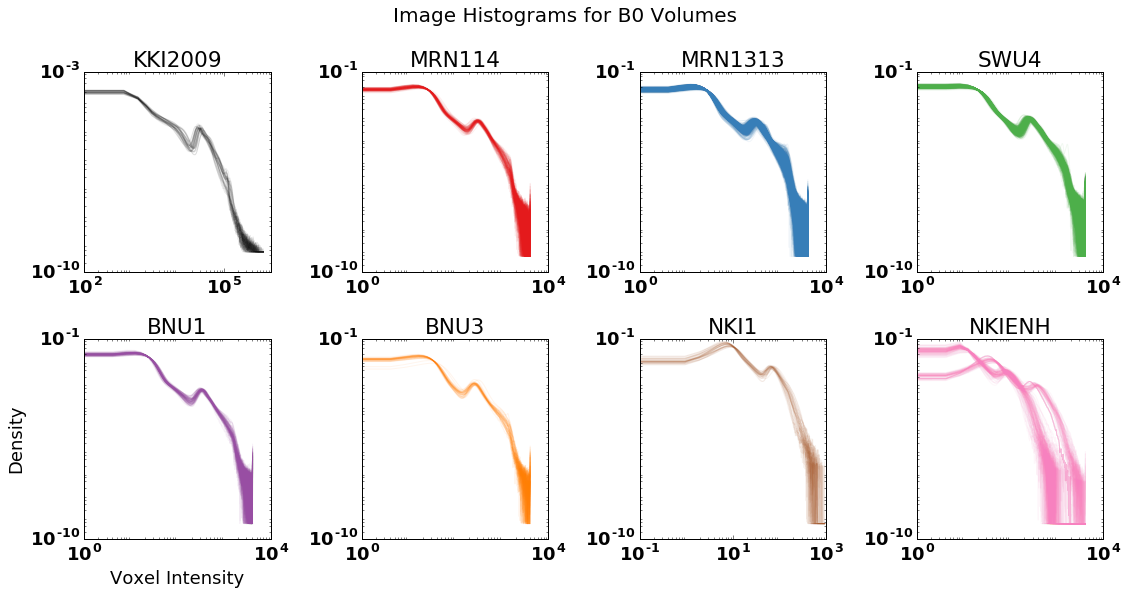
\includegraphics[width=1\textwidth]{multi_b0s_colourful.png}
\caption{An example comparison of summary statistics across different MRI datasets.
}
\label{f:mri}
\end{figure}



\begin{figure}%{l}{0.5\textwidth}
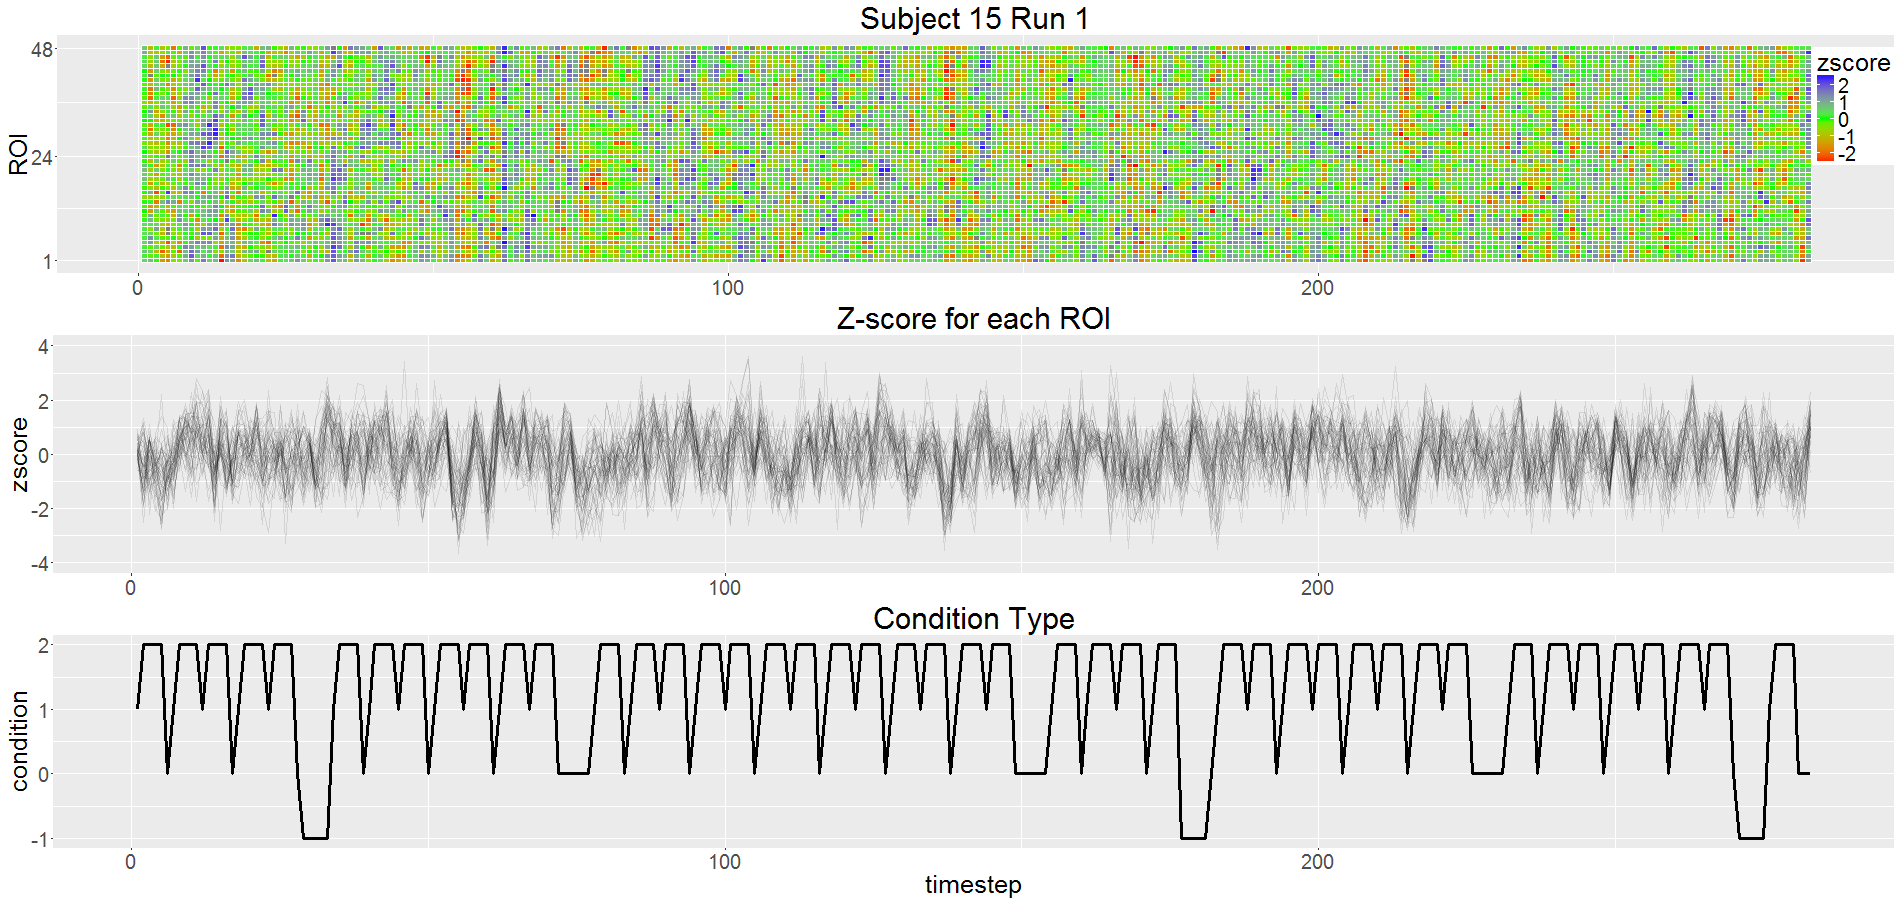
\includegraphics[width=1\textwidth]{sub-15_run1heat.png}
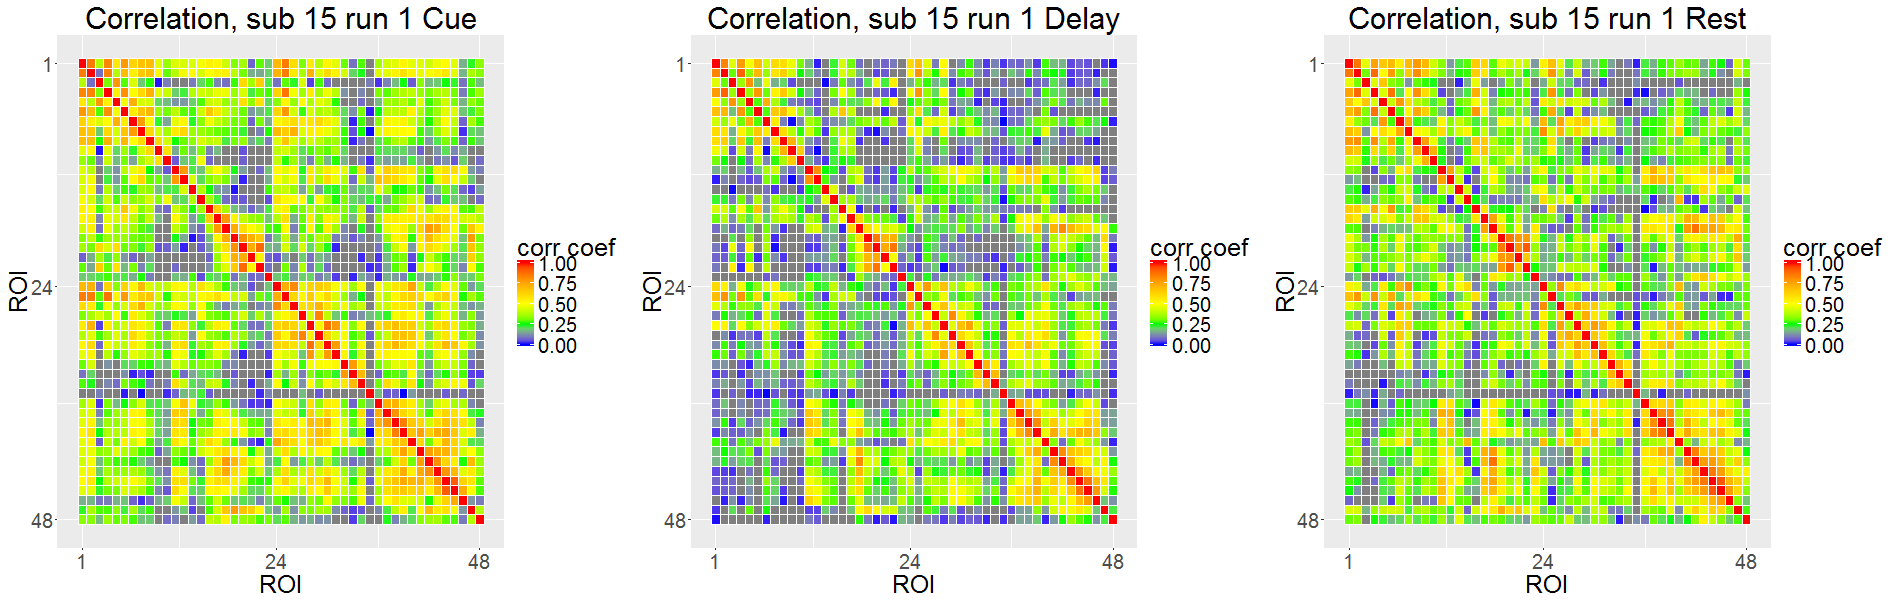
\includegraphics[width=1\textwidth]{sub-15_run1corr.png}
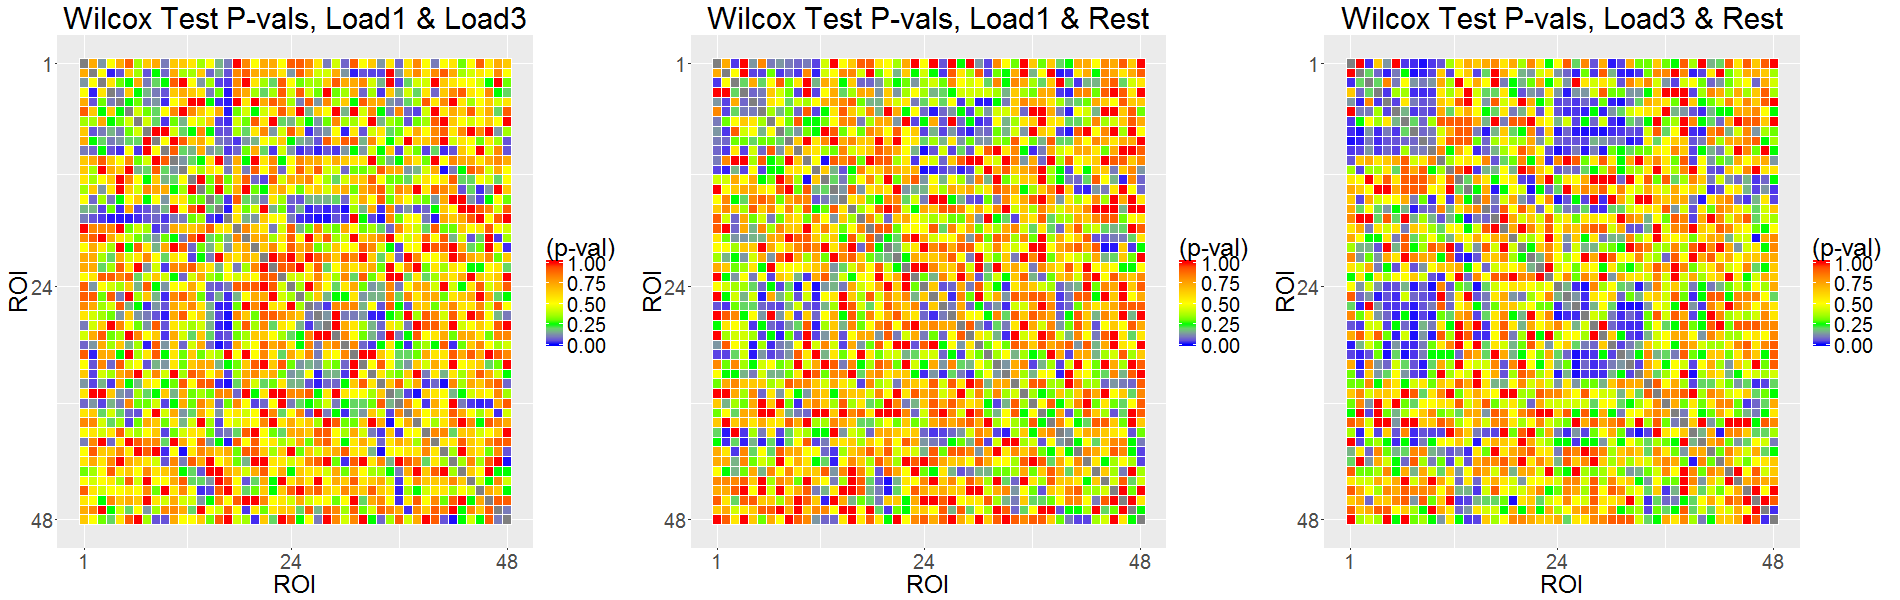
\includegraphics[width=1\textwidth]{overall_corr_wilcox.png}
\caption{An example dashboard for an physiology experiment.  Note that this dashboard could be effectively the same across a wide range of different experiments, spanning many different scales and domains.
}
\label{f:wilcox}
\end{figure}



\subsection{System Overview: Goal and Deliverables}

The project will develop a continuous-integration platform on top of NeuroData \cite{nd} and 
MRICloud that provide 
version control, data provenance, integrated testing, automated experiments, and analysis dashboards.  
A fundamental capability will be running controls against new data sources and updating experiments 
based on new inputs.  BrainLab CI will rely on software containers (e.g., Docker) 
to encapsulate the scripts and programs associated with a community experiment.  
Containers makes all scripts and programs {\em exactly repeatable} on different clusters and operating systems.  We will integrate containers with event-based serverless computing, 
such as Amazon Lambda, so that uploading new data to a community experiments triggers data controls and processing.  In this way, 
we can deploy BrainLab CI without any infrastructure investment, paying only for the computing that we use when we use it.

The project will {\bf deliver} a prototype CI system that accepts both physiology and MRI data that:
\begin{itemize}
\vspace{-7pt}
\addtolength{\itemsep}{-7pt}
  \item runs continuous experiments with community contributions and data acceptance criteria;
  \item supports inbound data processing based on serverless cloud computing as part of a data check in;
  \item supports refinement branch/fork of existing experiments;
  \item and, provides analyses and visualizations that reflect the outcome of the experiment for all versions. 
\vspace{-10pt}
\end{itemize}
We first describe the operation of the system, indicating how and when data processing and 
controls are triggered and run.  We then connect software components to cloud and HPC
architectures. 

%rhen, with an understanding of continuous integration for 
%neuroscience, we detail community experiments and data controls, clarifying how CI works 
%for data providers, community experiments, and open science reuse.

\para{Dataflow/Operational Architecture}
%
The design of BrainLab CI inherits from the service-oriented architectures 
that build continuous integration and continuous deployment into software repositories,
such as \textsf{GitHub} and \textsf{bitbucket}.
Both maintain a \emph{web hooks} API that invokes external services when events
occurs; for BrainLab CI, the events of interest will be (1) when new data are submitted 
to an experiment, (2) when experiments are cloned or pulled, and 
(3) when experiments are forked or branched.
We describe a few of the operations for a diffusion MRI example 
from the perspective 
%l and the system components that execute operations (Figure \ref{fig:op}(b)).
of a neuroscientist running an experiment (Figure \ref{fig:services}). We also 
connect each operation to the analagous git command.

\begin{figure}
  \begin{center}
    \hspace{-10pt}
    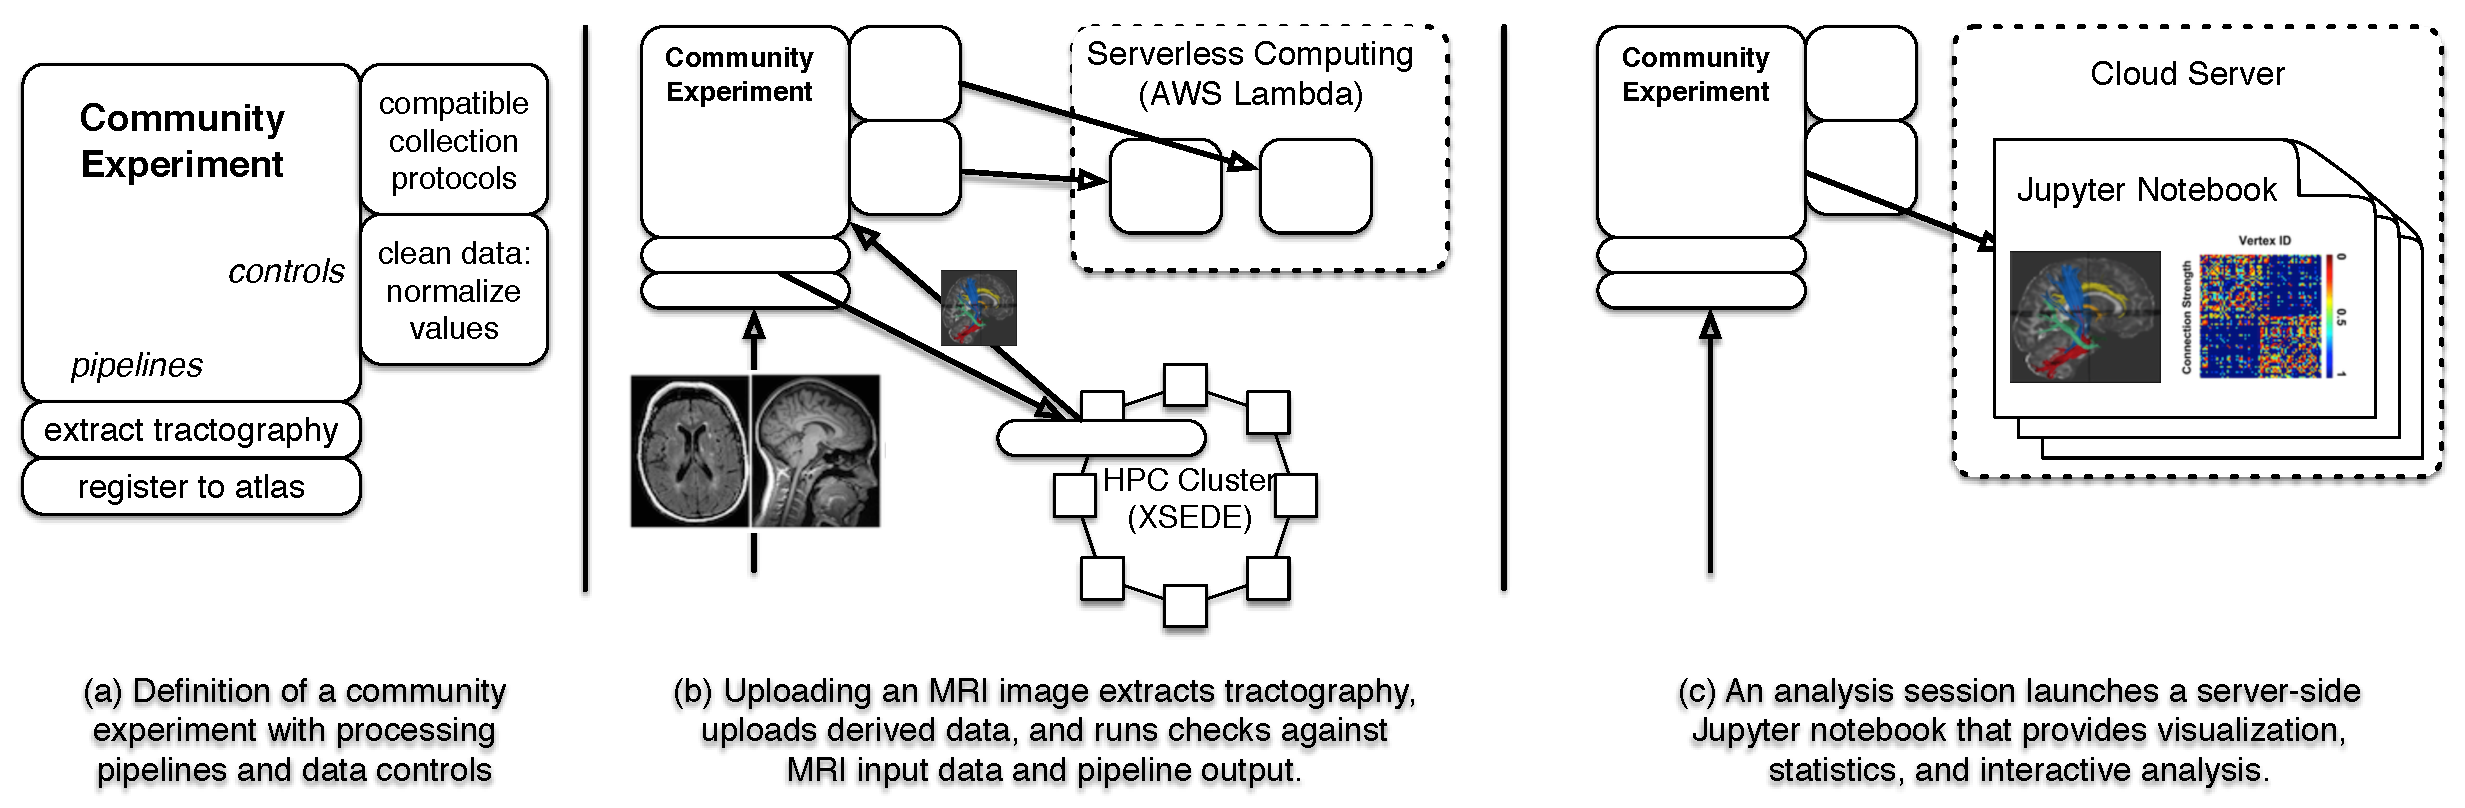
\includegraphics[width=6.7in]{blcifig.pdf}
  \caption{\small Overview of user interactions with a community experiment.}
  \label{fig:services}
  \end{center}
\end{figure}

% defining experiments
Users may define a community experiment (\textsf{git init}) or derive a new experiments 
from an existing experiment (\textsf{git branch} or \textsf{git fork}) using 
the management console at BrainLab CI.  (As with git, equivalent commands exist
for automation and power users.)  An experiment consists of a repository in which to 
place experimental data and metadata and a set of web hooks. 
For web hooks, users provide scripts or programs to be run on events that modify
the experiment or its data.  An experiment will also provide dashboards and 
vizualtions that generate and maintain the current state of results 
(graphs, tables, and figures).  Experiment owners create Jupyter notebooks to produce
these products that BrainLab CI runs automatically, as a web hook, when experimental
data change.

% webhooks/checks
When data are submitted to the users local version of a community 
experiment (\textsf{git commit}), BrainLab CI
invokes registered web hooks.  The example submits a NifTI file to the functional 
MRI experiment.  The first web hook checks whether the file has sufficient metadata and 
a conforming data (resolution and data type). 
%This is invoked as a serverless computation using Amazon 
%Lambda that runs in a Docker container. 
If the file passes input checks, the next
Web hook executes a preprocessing pipeline by submitted a supercomuting job to a
cluster, NSF XSEDE in this case.  This computation converts MRI imaging data into 
tractography data by stripping the skull from the image, registering the data to 
the Desikan atlas \cite{Desikan2006a}, and extracting neural pathways through white matter. Tractography data
are submitted back to the experiment and triggers a Webhook the updates local 
experimental result.

Subsequently, the user contributes these changes back to community experiment,
a \textsf{git push}.  The push Webhook updates the user's changes with the global
view, in this case using the same update routine that runs locally.
% pull/clone
Each user keeps experimental results consistent with the 
version of the experiment on which they are working.  Other user's contributions
do not automatically update their working version.  Users can update their
experiment (\textsf{git pull}) to merge in community contributions.  When 
they do so, a web hook will update their experiment.

Users may inspect and revert to past versions of the experiment
(\textsf{git checkout} and \textsf{git reset}).  For example, if the owner of
an experiment notices that data updates have produced inconsistent results
because data checks were insufficient.  They may revert to a previous good version
and add/modify the web hook routines that set criteria for data acceptance.
Users that do not own the experiment and wish to change web hooks must fork or 
branch the repository.

Analysis dashboards and visualizations are continuously updated, but their presentation are 
not linked to Web hooks.  Dashboards consist of graphs, statistics and visualizations
that are defined in Jupyter notebooks---a complete R/Python/Julia environment implemented
on the server.  When users access a notebook, they run the analyses in the notebook, materializing
the dashboard based on the most recent updates.  For a community experiment, the dashboard runs 
on the server and presents a uniform view to all.  For a forked, local or modified experiment the
dashboard runs locally based on all committed updates, whether they have been pushed or not.
 
\para{System Architecture}
%
We deploy Brainlab CI using a services-oriented architecture that eliminates systems
management and minimizes costs (Figure \ref{fig:services}).  Users enter our system 
through a Web application that provides the git-like experimental management Web services
and present analysis dashboards and visualizations.   For our prototype, we 
plan to develop on Amazon Web Services (AWS), although the system design is simply
portable to open-source clouds (OpenStack) and other providers (Google Compute Engine). 
The Web application scales elastically in an AWS scaling group, 
(de)commissioning servers based on demand.

We use serverless computing, with AWS Lambdas, for all continuous integration web hooks so that we
pay only for the computing that we use.  An AWS Lambda instantiates computing resources
on demand in response to a Web service request, e.g.~scripts that implement data controls 
on upload.

We link to supercomputers for compute-intensive tasks and long-running workflows, 
such as image processing, tractography for MRI, and cell detection and spike sorting for physiology.  
A Web hook will submit a supercomputing job
through an HPC scheduler (qsub, msub, or srun) and we launch a management task with 
the AWS Elastic Container Service to monitor/restart the job and move data back into the cloud when complete.

We use services for file and database storage, specifically AWS S3 and Dynamo respectively.

Taken altogether, BrainLab CI scales incrementally with usage from a minimum of 
a single Webserver to run permanent services up to an arbitrary number of resources on demand.


\subsection{Community Experiments and Data Controls}

Data controls allow data providers to set guidelines and restrictions on how data are reused.
Controls are defined in the context of an experiment, dictating what criteria data must meet 
to be included.  For a continuous or incremental community experiment, this concept is 
well-defined; the experiment owner sets the guidelines.

We are still developing the model for data reuse and derived experiments.  The challenge
is to balance data controls from the data owner with exploratory data mining and
ad-hoc reuse.  At one extreme, we could prevent anyone from using contributed data 
without inheriting all controls.  At the other, we could permit arbitrary reuse.  
Both are technically feasible.  The specifics of sharing will depend on the application
and domain and can be defined by the contributor.

We will implement and promote the concept of {\em compliant} and {\em non-compliant} data reuse, 
which permits ad-hoc usage, but also creates alerts for peer-review and auditing.
Compliant reuse inherits all experimental controls.  Non-compliant reuse allows derived
experiments or data reuse to add or remove controls.  In this way, there are no restrictions on 
exploratory data mining; anyone can use the data as they see fit.  However, unrestricted 
reuse flags an experiment as non-compliant, alerting data owners and reviewers to inspect 
the manner of reuse carefully.


\subsection{Broader Impacts}

BrainLab CI will create a prototype that will lead to a national and then global 
experimental infrastructure for neuroscience with the goal of breaking down barriers 
to data sharing and reuse.  The system eliminates objections to data sharing by 
allowing data contributors to implement controls on how data are used and audit/reproduce/rebut
experiments run against their data.  It also creates incentives to share data and use
the system for data providers.  Access to a large corpus of data will accelerate discovery and 
improve quality.  Thousands of subjects will reveal statistically significant trends not apparent in 
the data available from a single laboratory.  Larger studies that leverage community
data will become commonplace and then evolve to standard practice in neuroscience.

BrainLab CI democratizes access to neuroscience data, enfranchising a new class of scientists
that do not have the equipment, resources, or expertise to collect data. A larger, interdisciplinary
community will expand the set of ideas brought to bear on neuroscience and diversifying
the capabilities of the scientists that work on these data.  
Through tools like BrainLab CI, we can expand neuroscience beyond well-funded biomedical labs 
to a global community: to engage in brain science one needs a concept to explore and access to a 
Web browser.  We expect new ideas and new approaches to arise from the social, cultural, and 
intellectual diversity of an international community.

BrainLab CI will also form the basis for a richer type of citizen science in which 
citizen scientists perform data exploration and discovery based on their own 
curiosity.  This differs from existing approaches in which citizen scientists 
perform a specific, narrow task that contributes to a larger goal, such as 
galaxy spin and type classification in GalaxyZoo \cite{galaxyzoo} and tracing of neurons
in EyeWire \cite{eyewire}.  The data controls provide guidance as to how one can appropriately
combine data sets. 

BrainLab CI proposes a novel approach to community neuroscience.  It was conceived and feedback 
was taken from the neuroscience community during the NSF Global Brain Workshop.  This initial
design has garnered strong support from a network of collaborators (see Letters of Collaboration) that
include top research institutes (Allen and HHMI Janelia), academic labs (UNM, Stanford), and 
medical researchers (JHU Medicine and Child Mind Institute).  Additionally, we have taken feedback 
and will collaborate with European International efforts the Blue Brain Project and Human Brain 
Project (letter from Sean Hill).



\subsection{Suitability for EAGER funding}

%[NSF seeks] “…high risk/high reward innovative concepts and pilot projects that aim to ultimately result in deployment of ambitious, sustainable computational infrastructure resources, capabilities, and services that will enhance and accelerate the neuroscientific discovery process for a broad base of users.”
%While such solutions may require a degree of de novo development, NSF is particularly interested in supporting exploratory, pilot, and planning activities that emphasize maximal leveraging of existing shared computational infrastructure resources and capabilities…”

The project leverages existing community resources as well as cloud computing, allowing us to deploy 
continuous integration without developing new software infrastructure.
BrainLab CI builds upon the PIs' existing shared-infrastructure projects for storage, analysis, and 
pipeline processing of neuroscience data.  Time-series data 
(electrophysiology), 
spatial data (MRI and atlases), and spatiotemporal data (optophysiology and functional MRI) will be stored and managed 
in the NeuroData project (\url{http://neurodata.io}), formerly known as the OpenConnectome Project, 
which has been funded by an NSF/NIH CRCNS grant (1RO1EB016411-01), a BRAIN grant (1U01NS090449-01), 
and an NIH TRA (1R01NS092474-01).  
NeuroData includes built-in visualization and cloud data analysis based on Jupyter notebooks.  
MRI image processing, laboratory metadata, and registration will be provided by the 
NIH-funded MRI Cloud (\url{http://mricloud.org}), which uses 
NSF XSEDE computing (ACI-1053575) to provide scalable image processing to the open-science MRI community.

%“…identify and describe the immediate or anticipated need for the proposed computational infrastructure by one or more disciplines of brain science, and include at least one reference case or utilization scenario that will drive system requirements.”

BrainLab CI will fulfill an immediate need for integration, sharing and analysis for neuroscience data.
We have detailed two reference applications, MRI and neurophysiology.
The approach is general and applies to directly to other imaging modalities that take 
large numbers of subject each with modest data size.  These include MEG, EEG, ECoG, and PET.
Adapting BrainLab CI to other disciplines will require minimal software development. 
The core software remains that same; the difference among disciplines lies in encoding
domain expertise into, such as implementing data checks, processing pipelines, and
visualizations and analysis for dashboards.  These image modalities are used to understand 
and characterize a wide variety of neural disorders, including Alzheimer's, Parkinson's,
Autism, ADHD, and TBI.  

%“EAGER projects should be based on a strong, mutually dependent collaboration between neuroscientists and computational infrastructure developers/implementers, and should not include domain neuroscientific research activities other than those that are directly necessary to the technical effort.”

Brainlab CI builds upon two different, long-standing collaborations among 
computer scientists and neuroscientists, leveraging the tools built in both to create
new capability.  Neurodata has been run for five years by PIs Vogelstein and Burns
and has developed tools for curated data sharing and annotation of MRI, electron microscopy \cite{harris15}, 
CLARITY \cite{Chung2013a}, and Array Tomography \cite{weiler14} data.  NeuroData is a registered Nature data repository 
and hosts definitive, archival data sets for annotation, visualization and analysis.
MRICloud (\url{http://mricloud.org}), directed by Co-PI Miller, provides processing 
resources for the open-science MRI.  It provide the image processing and shape analysis 
capabilities of MRI studio 
(also developed by Miller) through Web-services, fulfilling computation for the services using 
the NSF XSEDE funded supercomputers.  


\subsection{Results from Prior NSF Support}


Burns has been the PI of five completed NSF-funded projects addressing high-performance data systems 
and scientific computing.   Award CCF-0937810 (12/15/09--12/14/13) developed throughput-oriented 
scheduling techniques for data-intensive clusters that preserve the performance of 
Web services when they scale out to support many users and large queries.  
The project resulted in four successive publications in the Supercomputing Conference from 2009--2013.
CAREER Award CCF-0238305 (5/1/03--4/30/08).  He was the PI of ``CAREER: Interoperation among Heterogeneous
Global-Scale Systems'' (NSF ACI-0238305, \$407,000, 3/15/03--3/14/08),  that built tools that manage the 
lifetime of data and allow information to flow seamlessly across management and software boundaries.  It lead
to more than 15 refereed conference and journal publications, including a Best Paper Award.

Burns has been the Co-PI of 7 interdisciplinary NSF grants that connect CISE and a science domain.
He has worked across turbulence with an ITR (2004-09) and two CDI awards (2010-2014,2015), 
astrophysics (2004-07, 2012-14, 2013-2018), and environmental engineering (2004-09).  He 
has had collaborative neuroscience funding since 2011 through the NIH and DARPA.

Burns has been PI for the joint NSF/NIH program Collaborative Research in Computational 
Neuroscience (NIBIB 1RO1EB016411-01).  Vogelstein was a Co-PI.  Burns and Vogelstein were
co-PIs on the joint NSF/NIH BIGDATA grant (NIDA 1R01DA036400-01).  

In addition, Vogelstein was PI for ``A Scientific Planning Workshop for Coordinating Brain Research Around the Globe''  (NSF, \$97,950, 04/01/2016 -- 03/31/2017), which coordinated the Global Brain Workshop 2016, from which these ideas emerged.  A perspective piece on the outcome of that meeting is currently under review at Science, and available from the workshop's website: \url{http://brainx.io/}.  The ideas in this proposal are very much a response to the discussions of that meeting.  Moreover, there are already three follow-up meetings scheduled for this calendar year, including a side event at the Unite Nations General Assembly to help the UN i
define grand challenges for global brain sciences.






\newpage
\setcounter{section}{5}
\setcounter{page}{1}
\rfoot{\small References Cited ~~ \thepage}

%\input{bibitems}
\setcounter{page}{1}
\small
\begin{spacing}{0.9}
\bibliographystyle{ieeetr}
\bibliography{blci,jovo}
\end{spacing}

\normalsize

\newpage

\renewcommand{\thepage}{\arabic{page}}
\setcounter{page}{1}
\rfoot{\small Data Management Plan ~~ \thepage}

\section*{Data Management Plan}


Our data management plan covers several distinct classes of data: 
\begin{itemize}
\addtolength{\itemsep}{-5pt}
\item neuroscience data contributed by the open science community,
\item software and documentation developed by the project team, and 
\item operational data, such as logging and usage statistics.
\end{itemize}
\vspace{-5pt}
All data sets will be archival; they are intended for long-term preservation and
subject to the data management policies described below.

This project is primarily conducted out of the KAVLI Neuroscience Discovery 
Institute.  Because it is a new institute, we are in the process of codifying 
data management principles.  We adopt the data management practices of 
the Institute for Data-Intensive Science and Engineering (IDIES) of which 
Burns, Vogelstein, and Miller are all active members.  IDIES aggregates the
data management and scientific computing exerptise at Johns Hopkins.

IDIES has successfully deployed data-intensive Web services that contribute 
computation and analysis to the public for several disciplines, including astronomy (sdss.org), 
computational fluids (turbulence.pha.jhu.edu), and connectomics 
(openconnecto.me). IDIES hosts more than 11 petabytes of contributed data in support of 
many disciplines.  IDIES has 13 years of experience 
hosting publicly accessible scientific databases and data-intensive Web-services. The best 
practices of the Institute will be adopted, as described below.

\subsubsection*{Licenses}
All scientific data sets will be released under the {\em Open Data Commons Attribution} (ODC-By) license.
The license allows for free use of all data products, including copying, sharing, and redistributing data, and
deriving new, customized data products.  Our specific license terms require that all subsequent
data use attributes the original publication that contributed the data as well as the project 
that hosts the data.  
All software and course material will be released under the Apache 2.0 license. This license is 
permissive; it places few restrictions on the use of software.
Derived software products or software systems that integrate our code or course materials 
do not need to be open-source.

\para{Documentation and Metadata} Source code documentation will be collocated and released with 
software, governed by the same open source license, and hosted on public repositories. 
Documentation for datasets are treated similarly. They 
will be managed in version control public repositories. They will be available as links that are 
collocated with the Web-services that provide access to data. These are already standard practices 
of the collaborators. 

\subsubsection*{Logging and Reporting Data}
We will use IDIES' extensive logging infrastructure to  track scientists
use data-intensive Web-services and supercomputing allocations in their research.
One of the most useful byproducts of the Sloan Digital Sky Survey  data has been the 
usage logs that we have kept since
the very beginning of the project: every Web hit and every single query have been logged since Day 1.
Today, the log database is over 2TB, and contains rich historical information about how astronomers
learned to access a virtual telescope. 
This has resulted in an amazingly rich and useful resource
for SDSS scientists and project managers and, because the dataset is available to anyone, many other
projects and researchers. IDIES has generalized this logging infrastructure for all projects.

Based on our logging infrastructure, we will be able to analyze the data usage patterns 
and contributions.  The goal is to inform the evaluation and reporting process 
with data-driven metrics at an arbitrarily fine granularity.  

\para{Data Integrity} IDIES systems make several efforts to ensure the integrity of the
 data and to prevent malicious or unintended modification. We use RESTful interfaces 
 for data access and to execute analysis routines, ensuring that all interfaces are functional and 
 do not modify the original data. For data stored at IDIES, we also regularly crawl our data 
 checking content against pre-computed checksums to protect against corruption from hardware and software errors. 
 For data stored in the Amazon cloud, we will rely on the integrity of AWS's data services. 
 

\para{Security, Privacy, and Embargo}
  The privacy of data sets is implemented with a combination of a user authentication in 
  our project management system and the secure Web-services (\url{https://}).  
  The combination allows users to self-manage access control to their data.  They may 
  set individual data sets, images, and annotation projects as public or private.
  Derived data products may be kept private by registered users of the system. 
  Private data sets will be encrypted end-to-end for all Web-services and visualization tools.

  The contributors of data maintain control of the data even after placing it in the system.
  They can determine when to make data public, when to release data from embargo, etc.

\para{Storage and Backup During the Project} The project builds a prototype that stores 
data in the Amazon Cloud.  Amazon provides guarantees about the reliability of data
in the service level agreements, e.g.~some data services implement triply redundant storage. 

\para{Long-Term Archival and Preservation}  While the goal of this project is to deploy a 
prototype, we will accumulate valuable data sets in doing so.  At the end of the project,
we will ingest these data sets in to the IDIES' storage infrastructure,
IDIES has preserved all scientific data that has 
  been ingested and will continue to do so in perpetuity. 
  The first resources developed were the Sloan Digital Sky Survey (sdss.org). 
  Multiple strategies have been used to maintain these data. We 
  have partnered with Google to store all image data on an ongoing basis. The development of 
  new data-intensive clusters (GrayWulf 2006 and Data-Scope 2012) has provisioned a small 
  fraction of resources to maintain the entirety of our previously collected data. Our preservation 
  ethic includes preserving the function and semantics of the data long after project operation 
  completes. We will do so by defining archival packages that include algorithms and methods as 
  well as data. We recognize sustainable preservation as one of the most challenging aspects of 
  developing data resources and note our commitment and experience in defining strategies to 
  fund and maintain resource-sharing beyond project lifetimes. 

\para{Data Sharing and Dissemination} This project focuses on making public datasets broadly 
available, leveraging the team’s expertise in storage systems and data 
processing to host scientific datasets for the nueroscience community.
This process makes data a community resource, greatly enhancing their 
utility. All public datasets referenced in this project will be available through Web-services. 

\para{Ownership, Copyright, Intellectual Property} Our projects encourages scientists and communities 
that ``open source'' their data in exchange for storage and analysis services. Open-source data 
becomes a community resource, unrestricted for non-commercial use. Data providers retain 
copyright privileges and reserve licensing and approval rights for commercial uses of data. 
Users of the data reserve rights to their algorithms and analysis techniques.



\end{document}


